\documentclass{beamer}
\usetheme{metropolis}
\title{LEGO Mindstorms Line Following Project}
\author{Aniruddha Pal, Markus Wiktorin}
\date{23rd of September 2016}
\institute{University of Applied Science, Bonn-Rhein-Sieg}
\begin{document}
	\maketitle
	\begin{frame}
		\frametitle{Task}
		Program a LEGO robot which can follow a line.
		
		Light conditions and track can change, the robot should work under different conditions.
	\end{frame}
	\begin{frame}
		\frametitle{Approaches}
		\begin{enumerate}
			\item One light sensor in front of the robot
			\item Two light sensors in front of the robot
			\item Two light sensors in front of the robot using PID
			\item Two light sensors, ultrasonic sensor and touch sensor in front of the robot using PID
		\end{enumerate}
	\end{frame}
	\begin{frame}
		\frametitle{1. Approach (one light sensor)}
		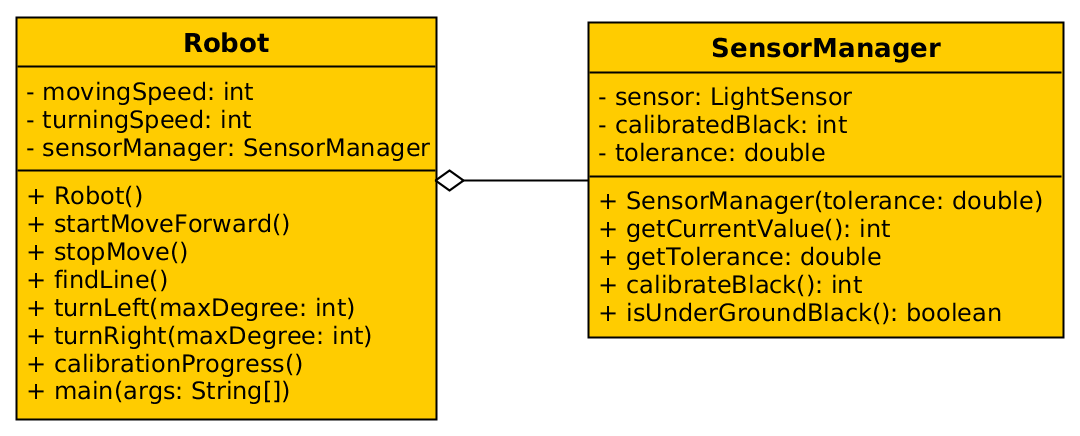
\includegraphics[width=\textwidth, height=\textheight, keepaspectratio]{firstApproach.png}
		\\
		Light sensor tries to stay in the middle of the line. If it looses the line it looks left and right in order to find it again.
		\\
		Bad approach but we tried to use object oriented concepts.
	\end{frame}
	\begin{frame}
		\frametitle{2. Approach (two light sensors)}
		\begin{itemize}
			\item We used two light sensors attached infront of the robot side  by side.
			\item The robot calculates the vakue difference of valus between the sensors.
			\item It takes left or right turn based on the difference of the two sensors.Also adjusts speed to take sharper turns.
			\item Advantage:
			\begin{itemize}
				\item Works better than the one sensor approach.
				\item Can take sharp turns
				\item Faster.
			\end{itemize}
			\item Disadvantage:
			\begin{itemize}
				\item Uses more power.
				\item Too much wear and tear of the motors. Harmful for it.
			\end{itemize}
		\end{itemize}
	\end{frame}
	\begin{frame}
		\frametitle{3. Approach (two light sensors + PID)}
		\begin{itemize}
			\item Same two sensor approach as the last one.
			\item Calculates the difference between the two motors which works as error value for proportional controller.
			\item Uses the previous error for better contol of movement. Integral approach.
			\item Appropiate values of Proportional, Integral and Differencial co-efficients used.
			\item Advantage:
			\begin{itemize}
				\item Less wear and tear of the motor. Works smoother.
				\item Is able to follow the track better.
			\end{itemize}
			\item Disadvantage:
			\begin{itemize}
				\item Finding out appropiate co-efficient values.
			\end{itemize}
		\end{itemize} 
	\end{frame}
	\begin{frame}
		\frametitle{4. Approach (two light, ultrasonic, touch sensor + PID)}
		\begin{itemize}
			\item We found some working values for PID in the third approach
			\item The robot is also fast on straights
			\item Next improvement: Make it possible to go on the same track with other robots
			\begin{itemize}
				\item Use ultrasonic in the front in order to detect other robots
				\item This was not working realiable, thats why we added the touch sensor
				\item The robot can still crash when it goes to turns, but on straights it is working good
			\end{itemize}
		\end{itemize}
	\end{frame}
	\begin{frame}
		\frametitle{Our robot}
		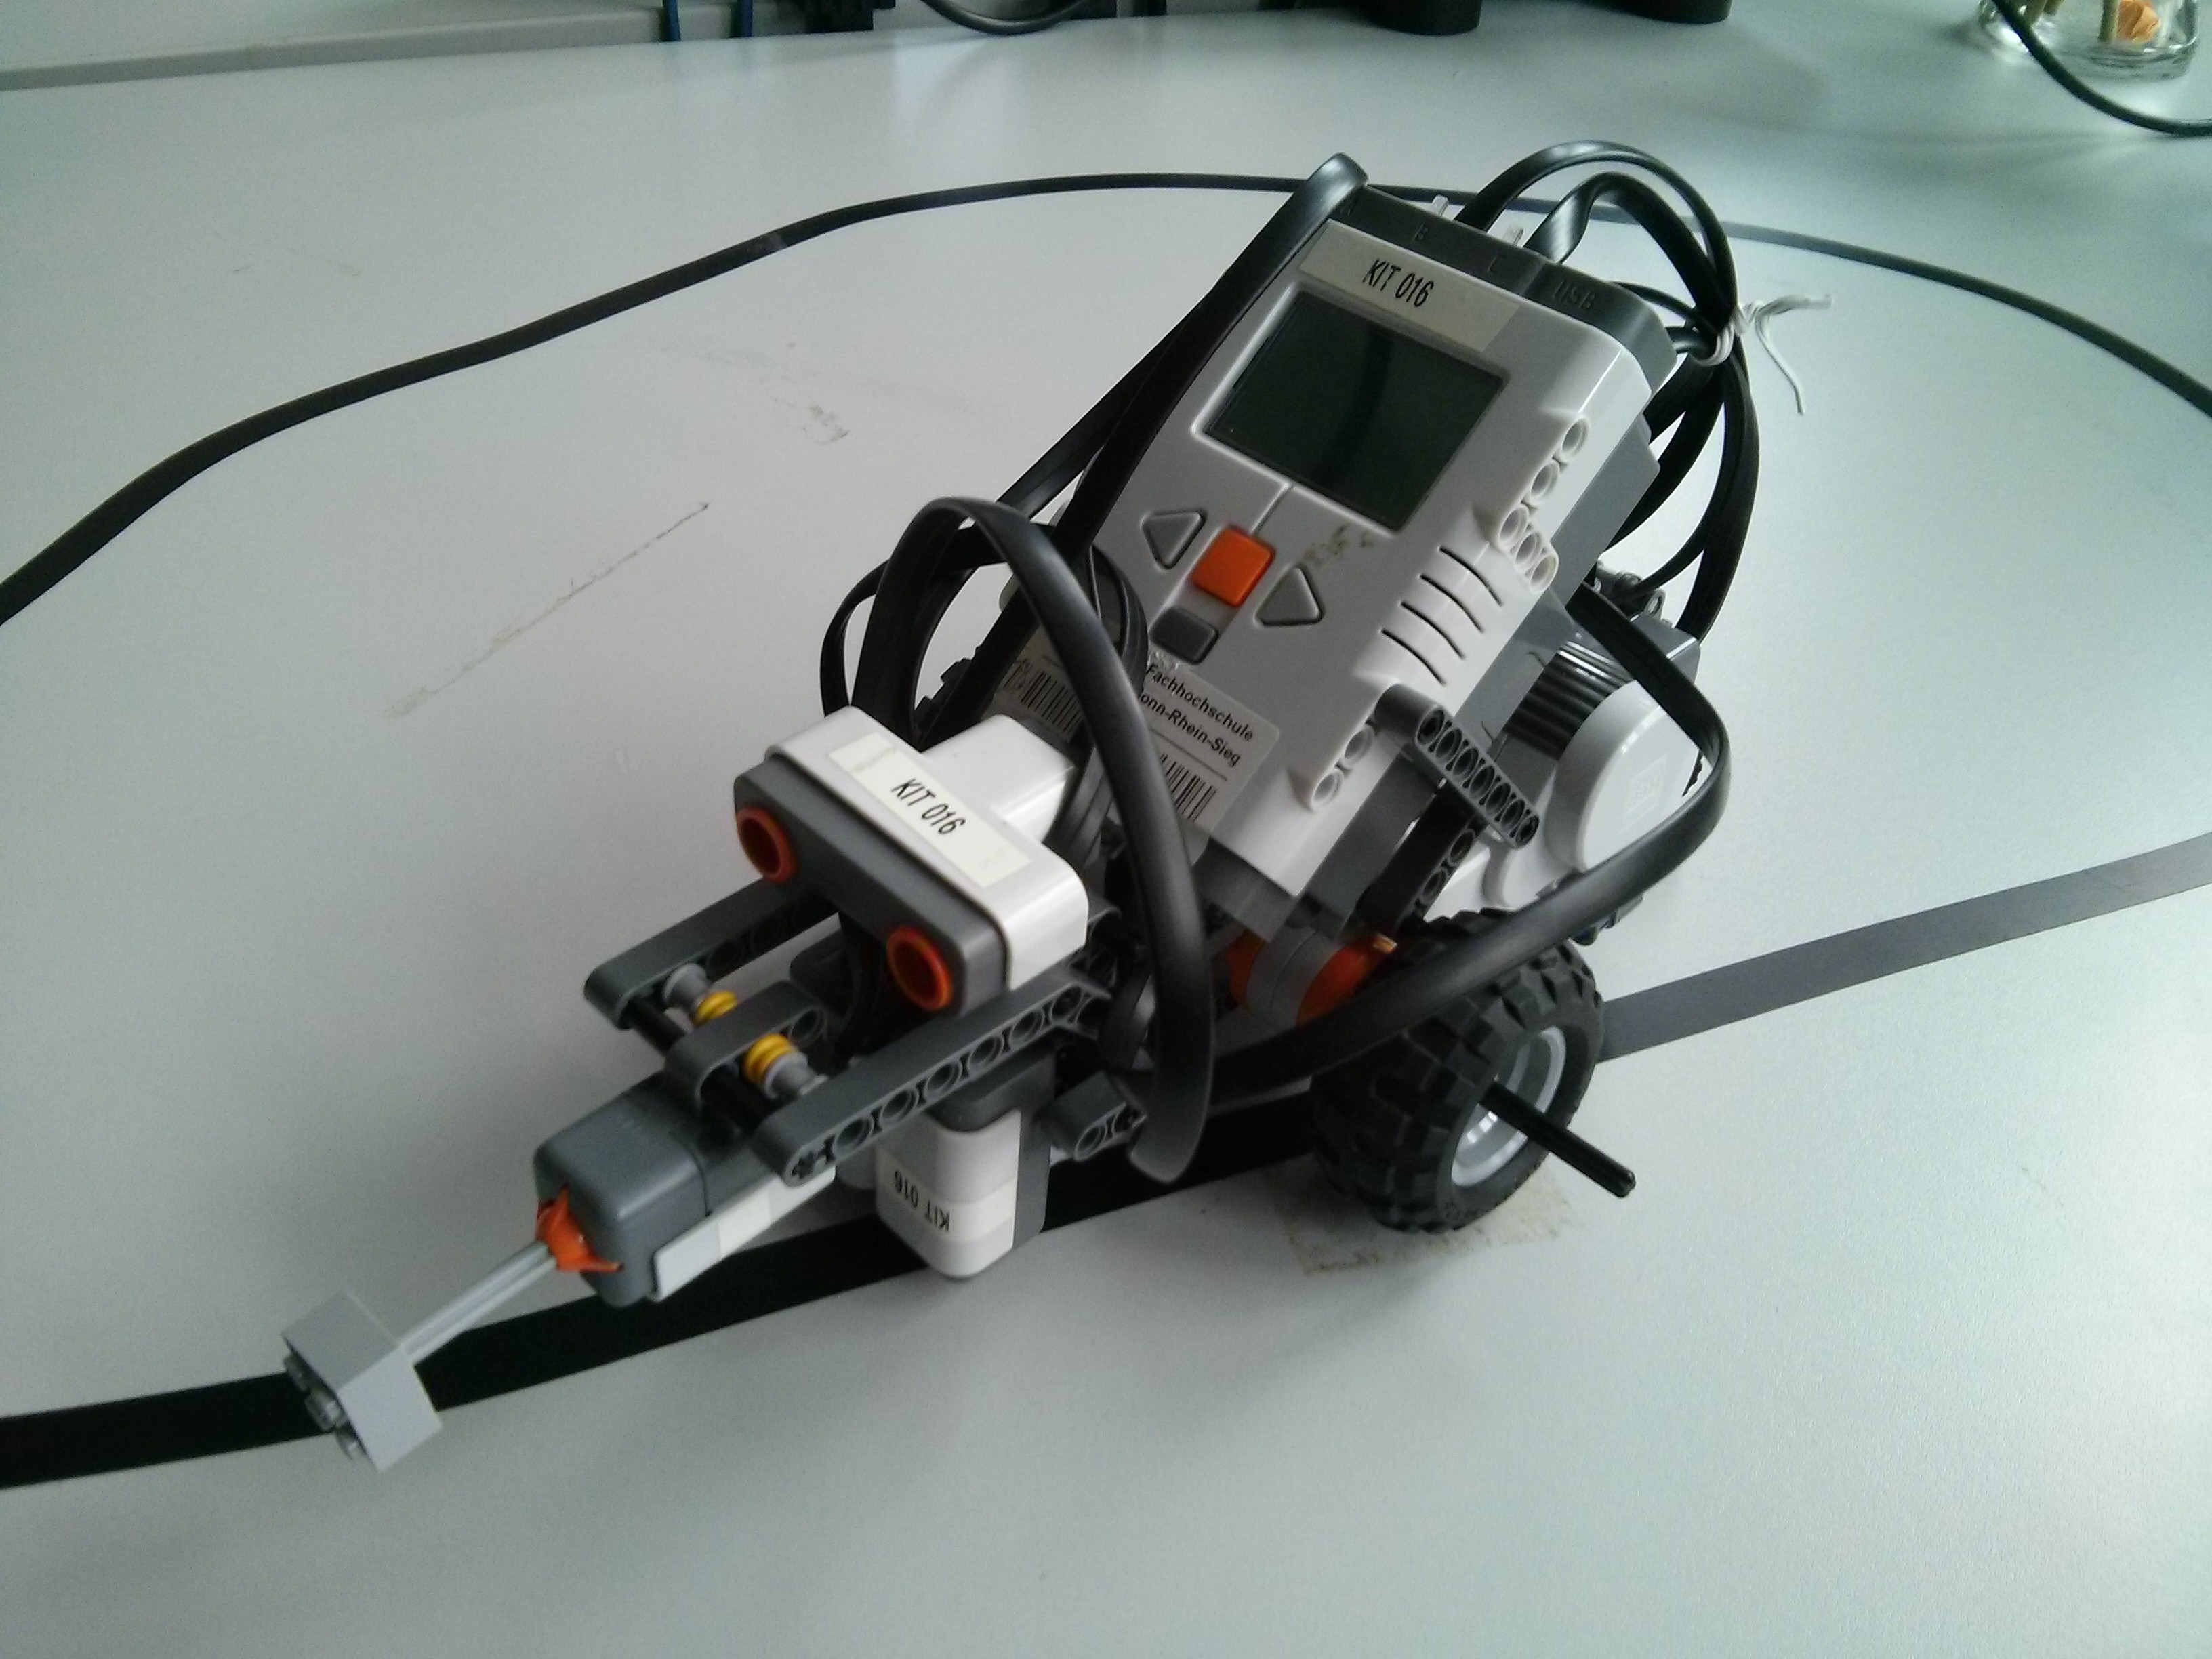
\includegraphics[width=\textwidth, height=\textheight, keepaspectratio]{IMG_20160922_170936.jpg}
	\end{frame}
\end{document}